
\documentclass[ms.tex]{subfiles}
\begin{document}

\section{Mock Samples}
\label{sec:mocks}

\begin{figure*}
\centering
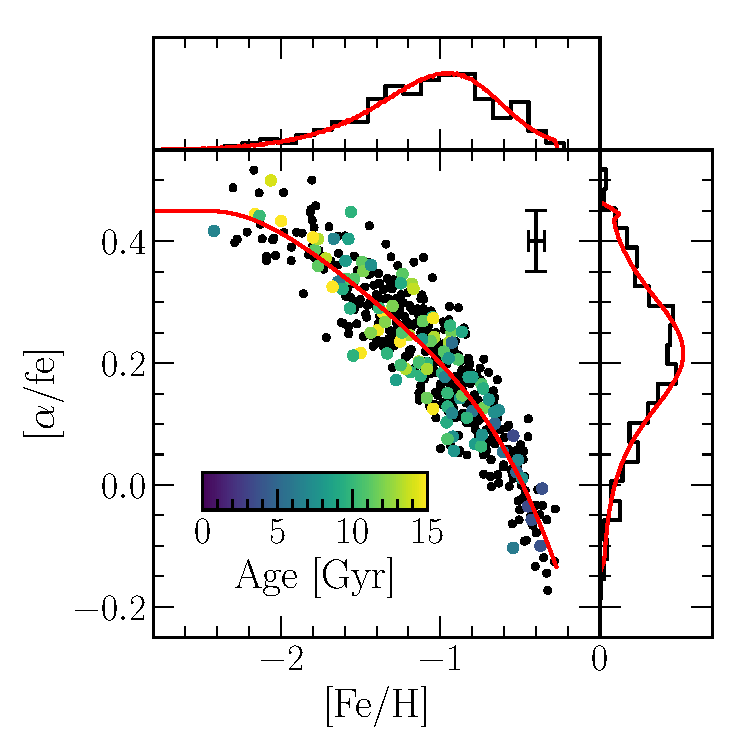
\includegraphics[scale = 0.5]{fiducial_mock_afe_feh.pdf}
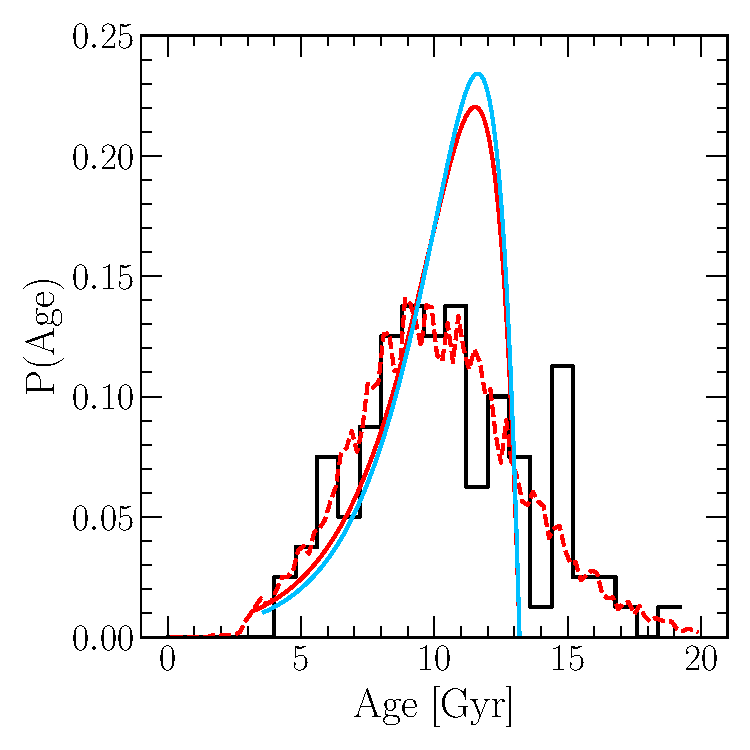
\includegraphics[scale = 0.42]{fiducial_mock_agedist.pdf}
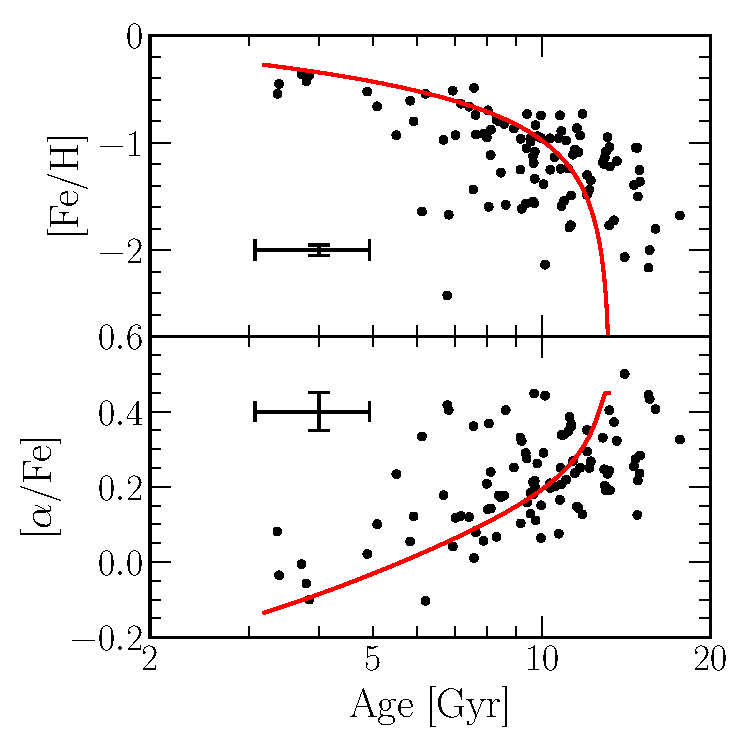
\includegraphics[scale = 0.42]{fiducial_mock_amr.pdf}
\caption{
\textbf{Left}: Our fiducial mock sample in the~\afe-\feh~plane.
There are~$N = 500$ stars with abundance uncertainties
of~$\sigma(\feh) = \sigma(\afe) = 0.05$ as indicated by the errorbar.
$N = 100$ of the stars have age information available with an artificial
uncertainty of~$\sigma(\log_{10}(\text{age})) = 0.1$ as indicated by the
colorbar.
The red line denotes the evolutionary track in the gas-phase from the one-zone
model that generated the mock.
On the top and right, we show the marginalized distributions
in~\afe~and~\feh, with red lines denoting the known distribution.
\textbf{Center}: The mock (black, binned) and known (red) age distributions.
The dashed red line indicates the age distribution that is obtained by sampling
$N = 10^4$ rather than $N = 500$ stars and assuming the same age uncertainty
of~$\sigma(\log_{10}(\text{age})) = 0.1$.
\textbf{Right}: The age-\feh~(top) and age-\afe~(bottom) relation for the mock
sample, with artificial uncertainties denoted by the error bars on each panel.
The red lines denotes the known relations for the gas-phase.
}
\label{fig:fiducialmock}
\end{figure*}

\begin{figure*}
\centering
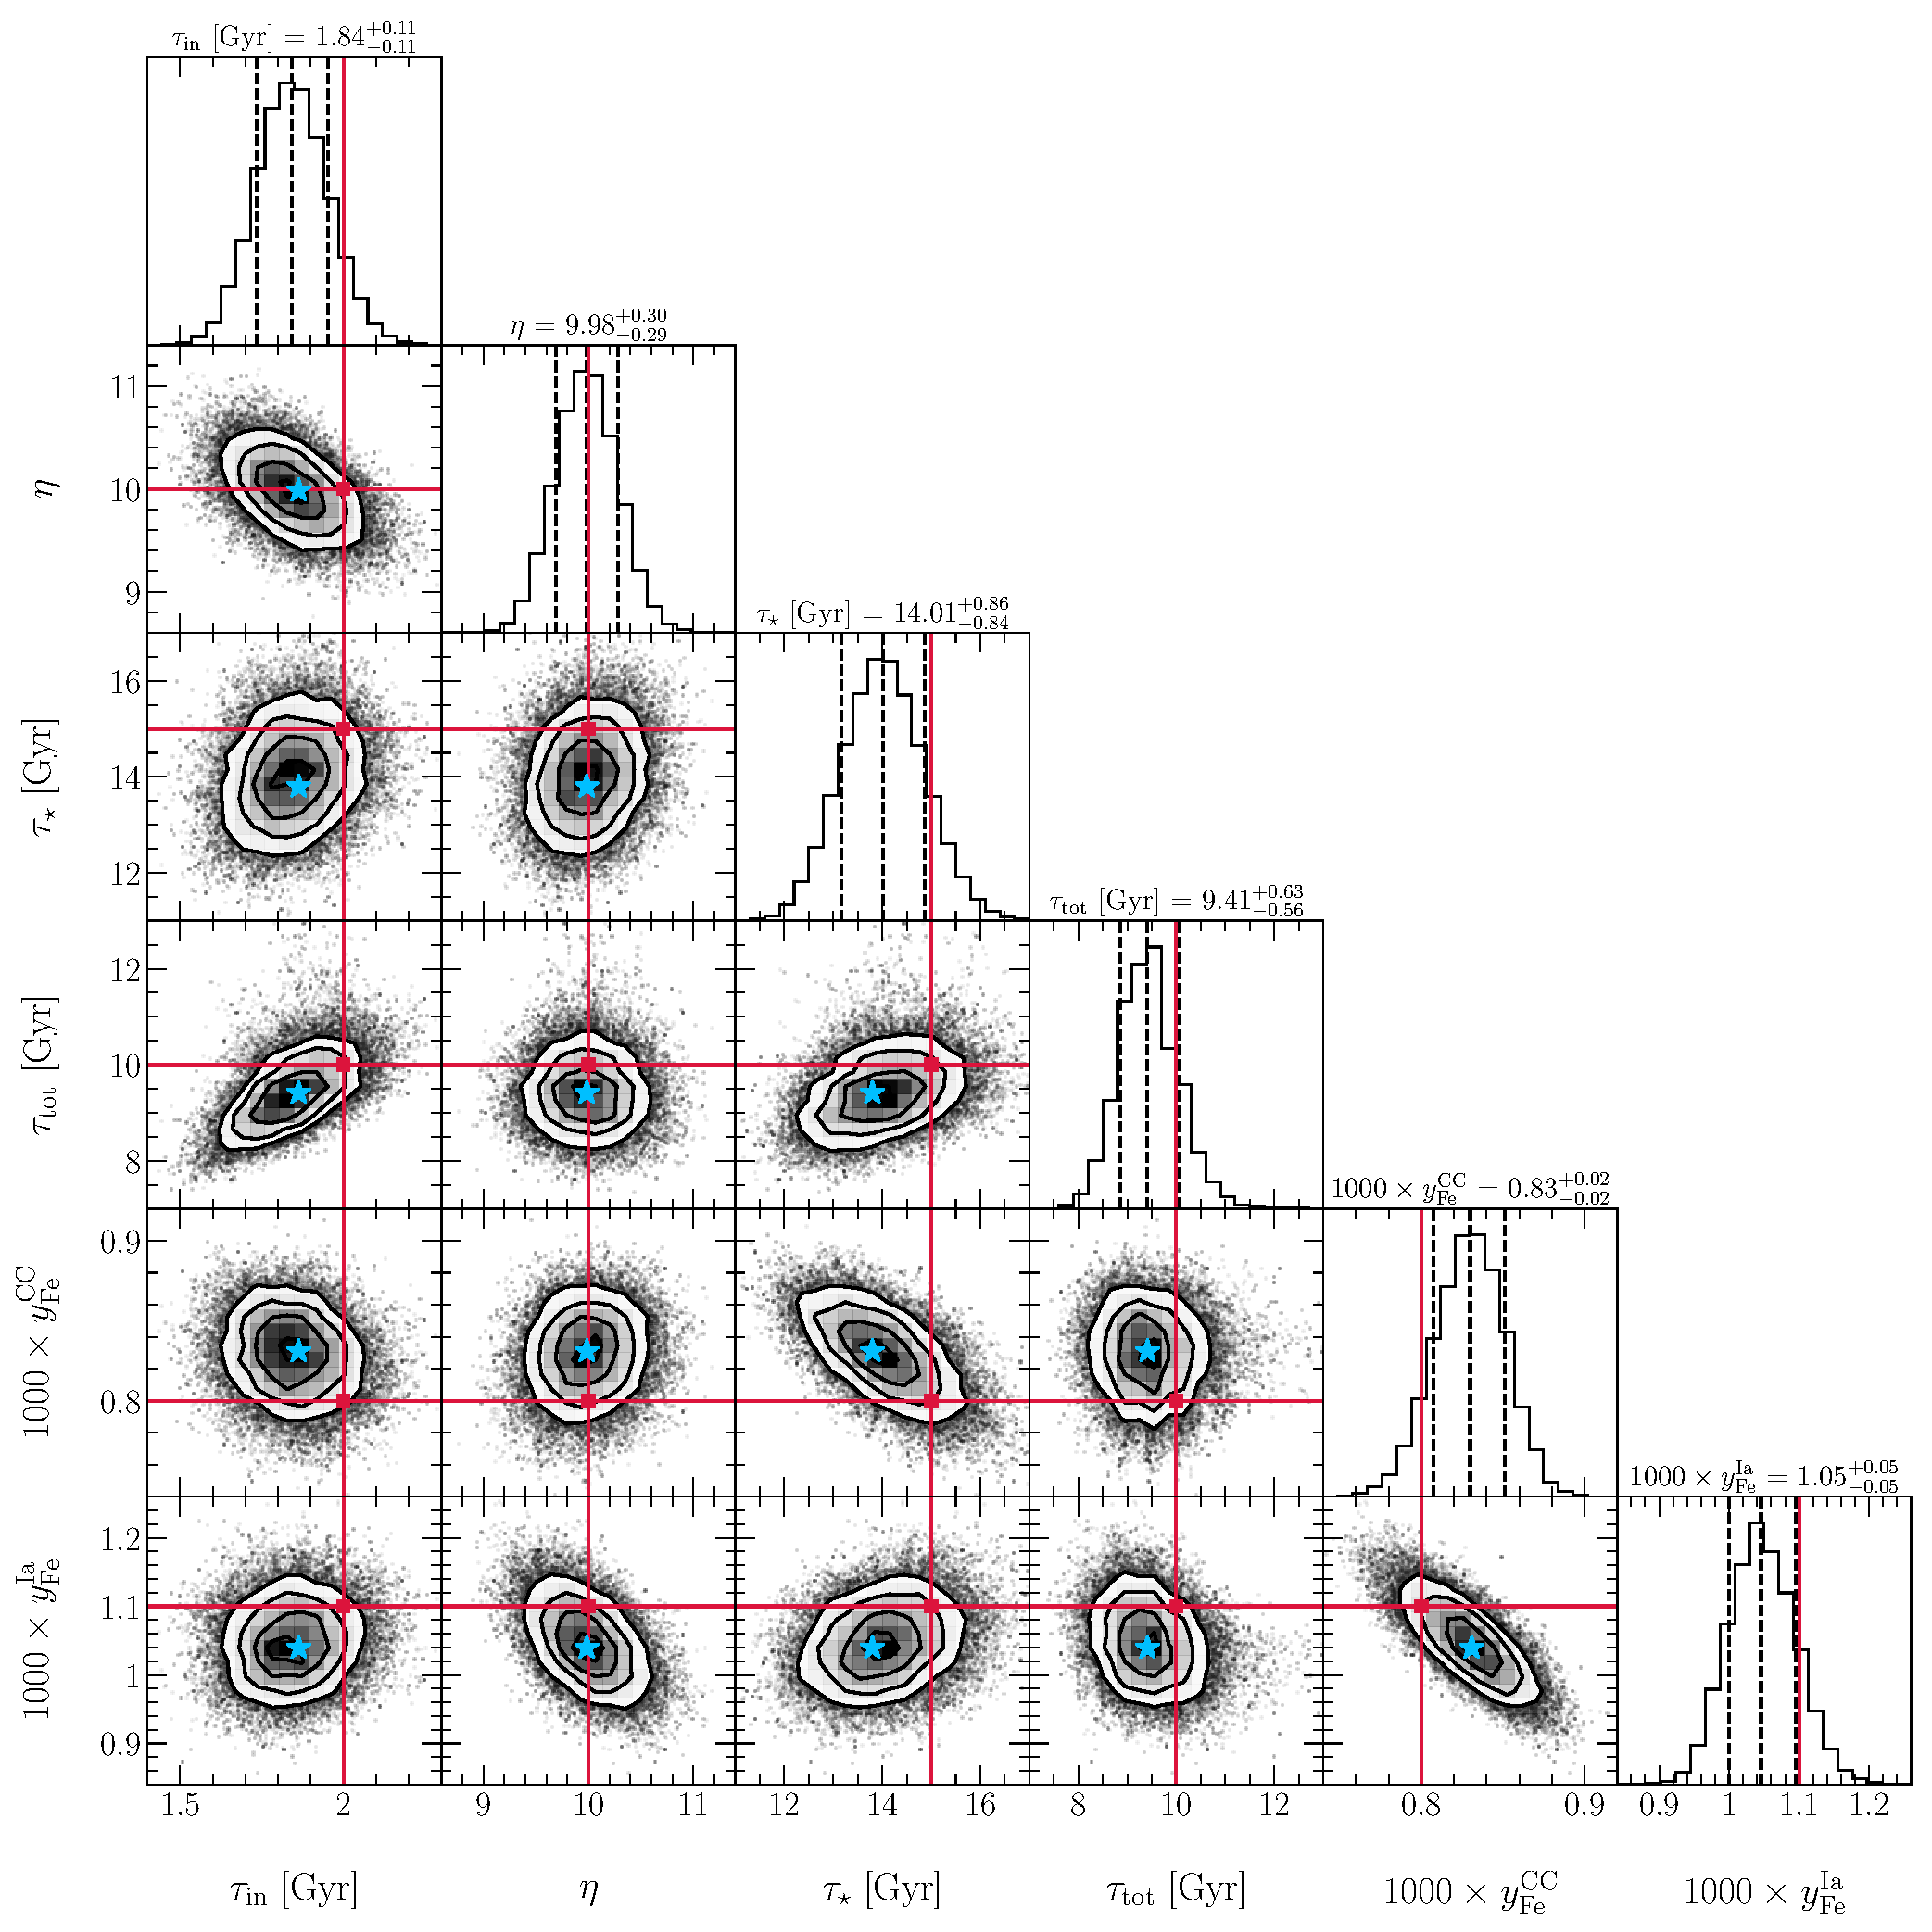
\includegraphics[scale = 0.45]{fiducial_76k8.pdf}
\caption{
The ``corner-plot'' showing the results of applying our fitting method to our
fiducial mock sample (see discussion in~\S\S~\ref{sec:fitting}
and~\ref{sec:mocks:fiducial}).
We show the marginalized likelihood distributions in each parameter along with
their best-fit values and confidence intervals along the diagonal.
Below the diagonal, we show the 2-dimensional cross-sections of the
6-dimensional likelihood function.
Blue stars mark the element of the Markov Chain with the maximum likelihood.
Red ``cross-hairs'' denote the true, known values of the parameters which were
used to generate the mock sample (see the top row of
Table~\ref{tab:recovered_values}).
}
\label{fig:corner_fiducial}
\end{figure*}

\subsection{A Fiducial Mock Sample}
\label{sec:mocks:fiducial}

\begin{itemize}

	\item Using our parametrization of one-zone GCE models described
	in~\S~\ref{sec:onezone}, in this section define a set of parameter choices
	from which mock samples of stars can be drawn.
	We then demonstrate the validity of our likelihood function (equation
	\ref{eq:likelihood}) in~\S~\ref{sec:mocks:fiducial_fit} by applying it to
	our fiducial mock sample and comparing the best-fit values to the known
	parameters from the mock.
	In~\S~\ref{sec:mocks:variations}, we then explore variations in sample
	size, measurement precision, and the availability of age information.

	% \item We use our parametrization of one-zone GCE models described
	% in~\S~\ref{sec:onezone} to set up an underlying model from which
	% mock samples can be drawn; we then use a fiducial mock sample to describe
	% our fitting method in~\S~\ref{sec:fitting} and explore variations
	% in, e.g., sample size and precision.

	\item We take an exponential infall hsitory~$\dot{M}_\text{in} \propto
	e^{-t/\tau_\text{in}}$ with an e-folding timescale of~$\tau_\text{in} = 2$
	Gyr and an initial ISM mass of~$M_\text{g} = 0$.
	We select an SFE timescale of~$\tau_\star = 15$ Gyr, motivated by the
	empirical result that dwarf galaxies have generally inefficient star
	formation~\citep[e.g.][]{Hudson2015}.
	We additionally select a mass-loading factor of~$\eta = 10$ because the
	strength of outflows should, in principle, contain information on the depth
	of the gravity well of a given galaxy, with lower mass systems being more
	efficient at ejecting material from the ISM.
	If the SFH in this model were constant, the analytic formulae of
	\citet{Weinberg2017} suggest that the equilibrium abundance of alpha
	elements would be~$\sim$16\% of the solar oxygen abundance, in qualitative
	agreement with the observed mass-metallicity relation for galaxies
	(e.g.~\citealp{Andrews2013, Tremonti2004};~\citealp*{Zahid2011};
	\citealp{Zahid2014}).

	\item With these choices regarding~$\tau_\star$ and~$\eta$, our parameters
	are in the regime where the normalization of the infall history, and by
	proxy the SFH, is inconsequential to the predicted evolution of the
	abundances.
	The appropriate likelihood function is therefore equation
	\refp{eq:likelihood} with normalized weights, whereas equation
	\refp{eq:lnL_withweights} with un-normalized weights would be the proper
	form if we had selected a parameterization in which the absolute scale of
	the infall history did impact the enrichment history.
	Inspection of the average SFHs predicted by the~\textsc{UniverseMachine}
	semi-analytic model for galaxy formation~\citep{Behroozi2019} suggests that
	the onset of star formation generally occurs a little over~$\sim$13 Gyr ago
	across many orders of magnitude in stellar mass.
	We therefore assume that the onset of star formation occurred~$\sim$13.2
	Gyr ago, allowing~$\sim$0.5 Gyr between the Big Bang and the first stars.
	We evolve this model for 10 Gyr exactly (i.e. the exact ages of the
	youngest stars are known to be~$\tau = 3.2$ Gyr), stopping short of 13.2
	Gyr because surviving dwarf galaxies and stellar streams in the Milky Way
	halo are known to have their star formation quenched
	\citep[e.g.][]{Monelli2010a, Monelli2010b, Sohn2013, Weisz2014a, Weisz2014b,
	Weisz2015} by ram pressure stripping from the hot gaseous halo
	\citep[e.g.][]{Steyrleithner2020}.
	These values are not intended to resemble any one galaxy, but instead to
	qualitatively resemble some dwarf galaxy whose evolutionary parameters can
	be re-derived using our likelihood function as a sanity check that it
	produces accurate best-fit parameters.

	% \item We take an exponential infall history described by
	% \begin{equation}
	% \dot{M}_\text{in} \propto e^{-t/\tau_\text{in}}
	% \end{equation}
	% with~$\tau_\text{in} = 2$ Gyr and an initial gas mass of 0.
	% The overall normalization of the infall history is irrelevant because
	% mass information cancels in one-zone models when you compute abundances.
	% We additionally select~$\tau_\star = 15$ Gyr and~$\eta = 10$ with the
	% thought that slow star formation and strong outflows would mimic the
	% evolution seen in a typical field dwarf galaxy.
	% We set the onset of star formation~$\tau = 13.2$ Gyr ago, allowing~$\sim$0.5
	% Gyr between the Big Bang and the first stars.
	% We evolve this model for 10 Gyr (i.e. the exact ages of the youngest stars
	% in the mock sample are~$\tau = 3.2$ Gyr).

	\item As discussed in~\S~\ref{sec:onezone:yields}, throughout this paper
	we assume that the IMF-averaged alpha element yields are exactly
	$\yacc = 0.01$ and~$y_\alpha^\text{Ia} = 0$.
	While loosely motivated by nucleosynthesis models in massive stars, this
	choice is intended to set some absolute scale of the effective yields.
	If no scale is assumed, then extremely strong degeneracies arise in the
	inferred yields, the strength of outflows~$\eta$, and the SFE timescale
	$\tau_\star$ due to the yield-outflow degeneracy (see discussion in
	Appendix~\ref{sec:yield_outflow_degeneracy} where we relax this assumption).
	The choice of~$\yacc = 0.01$ is intended to provide a round number from
	which the inferred parameters which are effected by this degeneracy can
	simply be scaled up or down to accommodate alternate parameter choices.
	In the present paper we do not distinguish between alpha elements because
	from a modelling standpoint they can all treated the same -- with a
	metallicity-independent yield from CCSNe and negligible yields from all
	other sources (at least for the lighter alpha elements such as O and Mg;
	\citealp{Johnson2019}).
	In practice, however, we take O as the canonical alpha element, adopting
	$Z_{\text{O},\odot} = 0.00572$ as the abundance of O in the sun accoring
	to~\citet{Asplund2009} and in agreement with the recent revisions of
	\citet*{Asplund2021},\footnote{
		We acknowledge that these values are in tension with constraints on the
		radiative opacity within the sun from helioseismology (i.e. the ``solar
		abundance problem'' -- see discussion in, e.g.,~\citealp*{Serenelli2011,
		Haxton2013, Bergemann2014}).
	} though similar~\afe~ratios would be predicted anyway if we instead took,
	e.g., Mg and asserted that [O/Mg]~$\approx 0$.

	\item \citet{Weinberg2017} adopt~$\yacc = 0.015$,~$\yfecc = 0.0012$ and
	$\yfeia = 0.0017$ (see discussion in their~\S~2.2).
	This massive star yield of Fe appropriate for nucleosynthesis models in
	which most~$M_\text{ZAMS} > 8~\msun$ stars explode as a CCSN
	\citep[e.g.][]{Chieffi2004, Chieffi2013, Nomoto2013, Woosley1995} assuming
	a~\citet{Kroupa2001} IMF.
	This SN Ia yield of Fe is based on the W70 explosion model of
	\citet{Iwamoto1999} which produces~$\sim0.77~\msun$ of Fe per SN Ia event
	and assuming that~$N_\text{Ia} / M_\star = \scinote{2.2}{-3}~\msun^{-1}$
	SNe Ia arise per solar mass of star formation based on~\citet{Maoz2012a}.
	Following this, we scale these values down by factors of~$\sim2/3$ such
	that $\yacc = 0.01$, adopting~$\yfecc = \scinote{8}{-4}$ and
	$\yfeia = \scinote{1.1}{-3}$ in our mock samples.
	We retain the assumption that~$\yacc = 0.01$ in our fits to our mock
	samples but otherwise let the Fe yields~\yfecc~and~\yfeia~be free
	parameters to be recovered by our likelihood function.
	We use this procedure in our application to the H3 survey
	in~\S~\ref{sec:h3} below as well.

	\item One-zone models as we have parametrized them predict simple stellar
	populations, so in order to construct a mock sample of individual stars, we
	must sample from the underlying SFH.
	High mass stellar populations have proportionally more stars than lower
	mass populations to contribute to some set of observations (this is also
	an important component of our fitting method; see discussion
	in~\S~\ref{sec:fitting}), so we take the probability of sampling a star
	from a given timestep to be proportional to the SFR at that timestep.
	We then sample~$N = 500$ stars each of which have -- in the interest of
	mimicking the typical precision achieved by a spectroscopic survey of a
	local group dwarf galaxy --~$\sigma_\afe = \sigma_\feh = 0.05$.
	100 of these stars have age information with an uncertainty
	of~$\sigma_{\logage} = 0.1$ (i.e.~$\sim$23\% precision).

	\item We illustrate this fiducial sample in Fig.~\ref{fig:fiducialmock}.
	This sample shows a ``knee'' in the~\afe-\feh~diagram near
	$\feh \approx -2.3$, and although the track extends to~$\feh \approx -0.3$,
	most of the stars form in the~$\feh \approx -1$ and~$\afe \approx +0.2$
	region of abundance space due to the declining nature of the SFH.
	In the next section below, we apply the likelihood function discussed
	in~\S~\ref{sec:fitting} to re-derive the known evolutionary parameters of
	this mock sample.

\end{itemize}

\subsection{Recovered Parameters of the Fiducial Mock}
\label{sec:mocks:fiducial_fit}

\begin{itemize}

	\item We apply the method outlined in~\S~\ref{sec:fitting} to the
	mock sample detailed in~\S~\ref{sec:mocks:fiducial}.
	Fig.~\ref{fig:corner_fiducial} shows the ``corner-plot'' derived from this
	procedure.
	Along the diagonal, we show the marginalized likelihood distributions in
	each parameter along with their best-fit values and confidence intervals.
	Below the diagonal, we show 2-dimensional cross-sections of the
	6-dimensional likelihood function.
	Blue stars mark the element of the Markov Chain with the highest value
	of~$\ln L$, and red ``cross-hairs'' denote the true, known values of the
	parameters from the mock sample (see the top row of
	Table~\ref{tab:recovered_values}).

	\item Our fitting method is able to accurately recover the known
	evolutionary parameters of the mock sample.
	Although it may appear that there are a high number of~$\gtrsim1\sigma$
	discrepancies, we demonstrate in~\S~\ref{sec:mocks:variations} that the
	differences between the known and best-fit values here are consistent with
	a Gaussian random process associated with measurement uncertainty.

	\item We note a handful of degeneracies in the likelihood distributions of
	the recovered parameters which arise as a consequence of having impact on
	the same observable.

	\begin{itemize}

		\item \textit{The centroid of the MDF.}
		With a fixed alpha element yield of~$\yacc = 0.01$ as we have adopted
		here, the strength of outflows~$\eta$ is set by ensuring the centroid
		of the~\ah~distribution is in agreement with the data.
		This in turn requires a total Fe yield~$\yfecc + \yfeia$ which
		corresponds to the centroid of the~\feh~distribution in the data.
		The total Fe yield, however, can be achieved with different breakdowns
		between CCSN and SN Ia enrichment.
		This gives rise to the inverse relationship between~\yfecc~and~\yfeia~as
		seen in Fig.~\ref{fig:corner_fiducial}.

		\item \textit{The position of the ``knee'' in the evolutionary track.}
		The ``knee'' in the~\afe-\feh~evolutionary track arises with the onset
		of SN Ia enrichment, a nucleosynthetic source of Fe but much smaller
		amounts of alpha elements.
		For fixed yields,~\citet{Weinberg2017} demonstrate that the SFE
		timescale~$\tau_\star$ plays the dominant role in establishing the
		value of~\feh~at which this occurs.
		With low~$\tau_\star$, star formation and consequently enrichment is
		fast, allowing the ISM to achieve a higher~\feh~before the onset of
		SNe Ia.
		However, with the CCSN Fe yield as a free parameter, agreement with the
		data can also be achieved with a higher (lower) value of~\yfecc~and
		slower (faster) star formation.
		This gives rise to the degeneracy between~\yfecc~and~$\tau_\star$ as
		seen in Fig.~\ref{fig:corner_fiducial}.

		\item \textit{The location of the track.}
		Any viable model which reproduces a galaxy's observed abundances in a
		self-consistent manner will predict a track that passes through the
		centroid of the 2-dimensional~\afe-\feh~distribution.
		With other parameters fixed, adjustments to the SN Ia Fe yield move the
		track vertically in the~\afe-\feh~plane (there is horizontal movement
		as well, but the vertical movement is a stronger effect).
		Conversely, the outflow mass-loading factor~$\eta$ is the most dominant
		evolutionary parameter in establishing the equilibrium abundance aside
		from the yields themselves.
		The tug-of-war between the source term of yields and the sink term of
		outflows establishing an equilibrium metallicity was demonstrated as
		early as~\citet{Larson1974} and again more recently
		by~\citet{Weinberg2017}.
		Adjusting~$\eta$ shifts the track horizontally in the~\afe-\feh~plane
		by changing the metal mass retained by the ISM.
		This gives rise to the degeneracy between~\yfeia~and~$\eta$: a change
		in parameter choices which shifts the track down and to the right (or
		up and to the left) may still achieve agreement with the data.

		\item \textit{The shape of the MDF.}
		The~\ah~and~\feh~distributions are affected in a handful of ways by
		these input parameters.
		For sharp infall histories (i.e. low values of~$\tau_\text{in}$), the
		predicted MDF is wider.
		This arises because with a sharp infall history, the gas supply also
		declines sharply with time, and consequently metals are deposited into
		a gas reservoir where the hydrogen and helium lost to star formation
		and outflows is not being replenished (for quantitative justification,
		see discussion in~\citealp{Weinberg2017}).
		These ``gas starved'' galaxies reach higher metallicities than what is
		achieved with a more steadily declining infall history, but a large
		fraction of their stars form early in their evolution when the
		abundances are low.
		As a result, the MDF is wider when~$\tau_\text{in}$ is small.
		\par
		While~$\eta$ establishes the equilibrium abundance in a galaxy for a
		given choice of yields, the SFE timescale describes the spped at which
		the galaxy reaches equilibrium~\citep{Weinberg2017}.\footnote{
			When star formation is fast, Fe is instead limited by the
			timescales associated with the SN Ia DTD, but in the dwarf galaxy
			regime, star formation is generally slow, and it is known to be so
			in this mock sample.
		}
		As a consequence, for a given duration of star formation, a galaxy
		spends less time near its equilibrium abundance when its inefficient at
		forming stars, an effect which increases the weight of low~\feh~stars
		in the MDF.
		Lastly, the duration of star formation~$\tau_\text{tot}$ has the effect
		of cutting off the MDF at some abundance quite literally by stopping
		star formation.
		\par
		Folding all of this together, degeneracies between these parameters
		arise as a consequence of their effects on the MDF.
		Between~$\tau_\text{in}$ and~$\tau_\text{tot}$, a sharp infall history
		can broaden the MDF, but stopping star formation early can cut off the
		MDF, allowing it to retain a peaked shape if the data suggest it.
		Between~$\tau_\text{in}$ and~$\eta$, a sharp infall history increases
		the equilibrium abundance, shifting the centroid of the MDF, but it can
		be lowered by increasing the strength of outflows.
		Between~$\tau_\text{tot}$ and~$\tau_\star$, a fast approach to
		equilibrium can cause the MDF to take on a strong peak, but if star
		formation is stopped early, the frequency of near-equilibrium stars is
		truncated, allowing it to retain a broader shape if the data suggest it.
	\end{itemize}

	% \item There are additional, weaker degeneracies which can be understood
	% by confounding variables.
	% For example, the degeneracy between~$\tau_\star$ and~\yfeia~arises because
	% both are degenerate with~\yfecc.

	\item We remind the reader that our fits achieve such a precision by
	selecting a scale on which the~$\alpha$ element yield~\yacc~is defined to
	be exactly 0.01 (see discussion in~\S~\ref{sec:onezone:yields}).
	Aside from the infall timescale~$\tau_\text{in}$ and the total duration of
	star formation~$\tau_\text{tot}$, each parameter in this fit is affected by
	the yield-outflow degeneracy.
	When~\yacc~is introduced as an additional free parameter, the likelihood
	function becomes extremely degenerate (see discussion in Appendix
	\ref{sec:yield_outflow_degeneracy}).
	The infall timescale and duration of star formation are not affected by
	this degeneracy because they affect only the shape of the MDF, an
	observational diagnostic which is constrained by a sufficiently large
	sample.

	\item To quantify the quality of the fit, for each datum~$\script{D}_i$
	we find the point along the track~$\script{M}_j$ with the maximum
	likelihood of observing the datum (i.e.~$\{\script{D}_i, \script{M}_j |
	\ln L(\script{D}_i | \script{M}_j) = \max\left(\{
	\ln L(\script{D}_i | \script{M})\}\right)\}$).
	We then base our value of~$\chi^2$ off of the vector differences
	$\Delta_{ij} \equiv \script{D}_i - \script{M}_j$ between the two according
	to $\chi^2 = \sum_{i,j} \Delta_{ij}C_i^{-1}\Delta_{ij}^T$ where~$C_i^{-1}$
	is the inverse covariance matrix~$C_i$ of the~$i$'th datum.
	We divide~$\chi^2$ by the sample size minus 6 (the number of free
	parameters in the GCE model) to estimate the~$\chi^2_\text{dof}$ statistic
	to assess the quality of the fit.
	Although we find that marginalizing over the track~\script{M}~is necessary
	to derive accurate best-fit parameters (see discussion
	in~\S~\ref{sec:fitting}), pairing each datum with a point on the track
	should be a safe estimate of the quality of the fit.
	As noted in the middle panel of Fig.~\ref{fig:fiducialmock}, our method
	achieves~$\chi_\text{dof}^2 = 0.55$, indicating that we have perhaps
	over-parametrized the mock data.
	This is unsurprising, because in the interest of demonstrating its
	reliability we have fit the mock data with the exact, known parametrization
	of its evolutionary history and nucleosynthetic yields with accurate
	estimates of the uncertainties.

	\item These tests against mock samples demonstrate the importance of
	the two central features of our method -- weighting the likelihood by the
	SFH and marginalizing over the track for each datum (see discussion
	in~\S~\ref{sec:fitting}).
	When either the weights or the marginalization are excluded from the fit
	procedure, the method fails to recover the evolutionary parameters with
	discrepancies at the many-$\sigma$ level between the best-fit and known
	values.
	For this reason, we caution against the accuracy of GCE parameters which
	are inferred from simpler likelihood estimates, such as matching each datum
	with the nearest point on the track.

\end{itemize}

\subsection{Variations in Sample Size, Measurement Precision, and the
Availability of Age Information}
\label{sec:mocks:variations}

\begin{figure*}
\centering
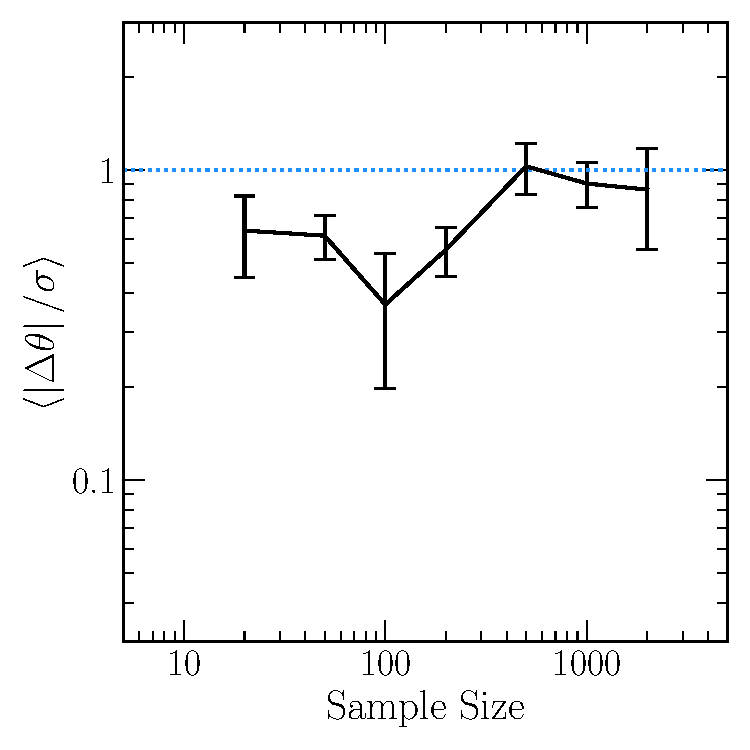
\includegraphics[scale = 0.45]{dp_sigma_samplesize.pdf}
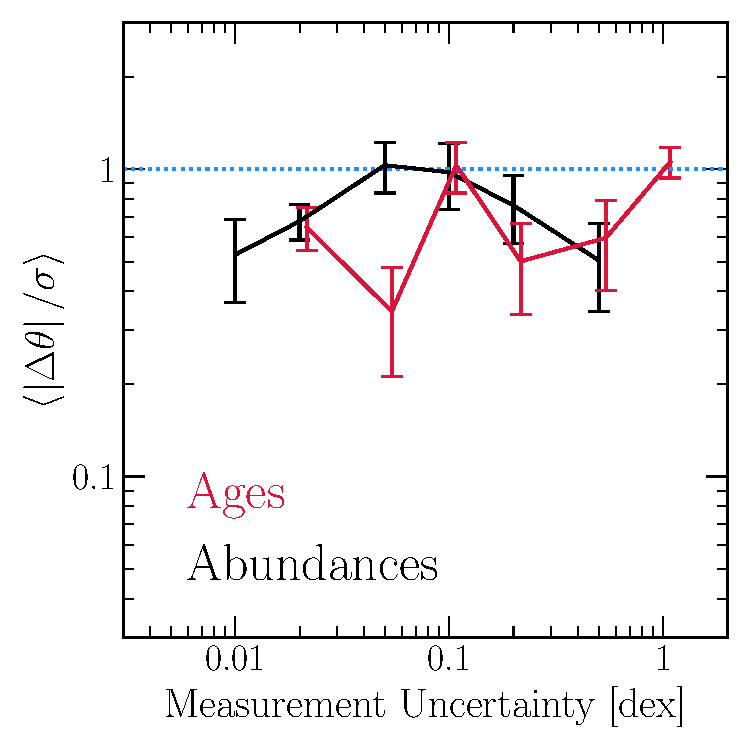
\includegraphics[scale = 0.45]{dp_sigma_precision.pdf}
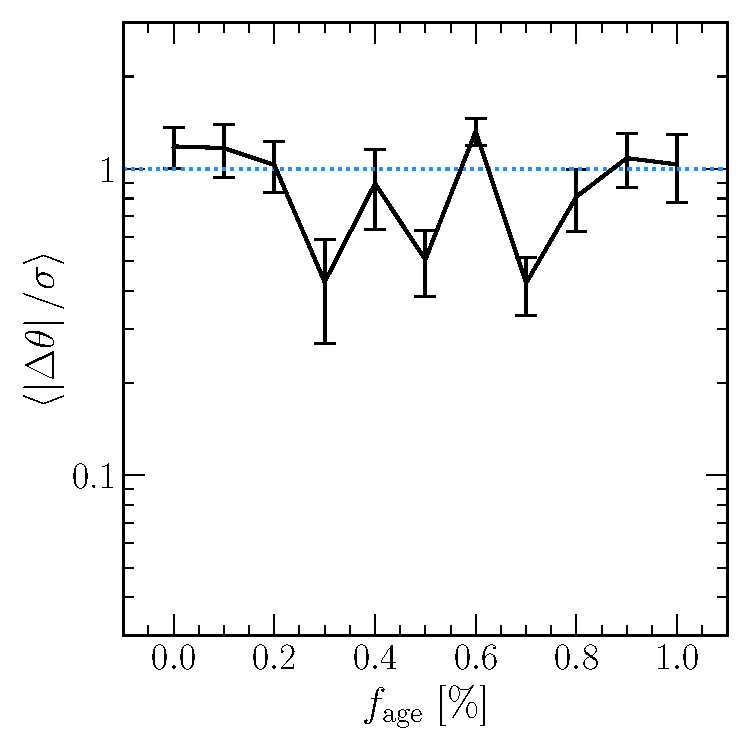
\includegraphics[scale = 0.45]{dp_sigma_agefrac.pdf}
\caption{
The mean deviation between the re-derived mock sample parameters~$\{\theta\} =
\{\tau_\text{in},~\eta,~\tau_\star,~\tau_\text{tot},~\yfecc,~\yfeia\}$ and
their known values from the mock sample in units of the uncertainty on the
best-fit values as a function of the sample size of the mock (left),
measurement precision in abundances~\feh~and~\afe (middle, black),
measurement precision in~$\log_{10}(\text{age})$ (middle, red),
and the fraction of the sample with available age information (right).
Error bars denote the error on the mean deviation in the six parameters.
Blue dotted lines mark~$\langle\Delta\theta/\sigma\rangle = 1$, the
expected value of the mean deviation for a Gaussian random process.
}
\label{fig:dp_sigma}
\end{figure*}

\subfile{mocksamples.tablebody.tex}

\begin{itemize}

	\item We now explore variations of our fiducial mock sample with respect
	to sample size, measurement precision, and the availability of age
	information.
	These variations retain all of the evolutionary parameters of the fiducial
	mock, but differ in one of the number of stars in the sample, measurement
	uncertainty in~\feh~and~\afe~abundances, measurement uncertainty
	in~$\log_{10}(\text{age})$, or the fraction of the sample with age
	measurements.
	The left-hand column of Table~\ref{tab:recovered_values} provides a summary
	of the values we take as exploratory cases for each mock variation, with
	the values taken in the fiducial sample highlighted in bold.
	In the remaining columns, we provide the associated values derived for each
	GCE parameter~$\theta$ along with their~$1\sigma$ uncertainties; the true
	values are noted in the top row.
	Our choices in measurement precision are intended to reflect typical values
	achieved by modern spectroscopic surveys where robust age information is
	often available for only a portion of the sample, and may be adopted from
	another source with a precision that is unrelated to the abundance
	uncertainties.
	Our chosen sample sizes are also intended to reflect a typical sample that
	might accurately be described by a one-zone model; with the requirement
	that mixing be efficient, it is likely that only dwarf galaxies meet this
	condition (see discussion in~\S~\ref{sec:onezone}).
	Much more distant than nearby Galactic stars and intrinsically smaller,
	dwarf galaxies are less conducive to the large sample sizes achieved by
	surveys of the Milky Way such as APOGEE\footnote{
		Apache Point Observatory Galaxy Evolution Experiment
	}~\citep{Majewski2017}and GALAH\footnote{
		GALactic Archaeology with Hermes
	}~\citep{DeSilva2015, Martell2017}.
	% In larger systems like the Milky Way, processes such as stellar migration
	% (refs) and radial gas flows (though perhaps less importantly; refs) have
	% been demonstrated to significantly impact the observed abundance
	% distributions as well as their evolution.
	% This demands a more sophisticated parametrization than a one-zone model
	% anyway, prompting a number of authors to explore so-called ``multi-zone''
	% GCE models (refs).

	\item Fig.~\ref{fig:dp_sigma} demonstrates the accuracy of our fitting
	method with respect to variations in these details surrounding the data.
	We compute the deviation between each re-derived paramter~$\theta$ (i.e.
	$\tau_\text{in}$,~$\eta$,~$\tau_\star$, etc.) and its known value, then
	divide by fit uncertainty~$\sigma_\theta$, and plot the mean for the
	corresponding sample on the y-axis.
	Under all mock variants that we explore, our method recovers the known
	values of the parameters to~$\sim1\sigma$ or slightly better.
	This is exactly as expected when the uncertainties are described by a
	Gaussian random process, wherein the most likely deviation from the true
	value is exactly~$1\sigma$.
	This is true even with infinite data, though in that limit the~$1\sigma$
	uncertainty interval becomes arbitrarily small.
	% \footnote{
	% 	The most likely value drawn from a normal distribution is exactly
	% 	$1\sigma$ from the mean.
	% 	The recovered values should also be consistent within~$1\sigma$ only
	% 	68.2\% of the time and discrepant at the~$>1\sigma$ level the remaining
	% 	31.8\% of the time.
	% }

	\item This suggests that our method should provide accurate best-fit
	evolutionary parameters even when the sample size is as low
	as~$N \approx 20$, when the measurement uncertainties are as high
	as~$\sigma_\text{[X/Y]} \approx 0.5$ and~$\sigma_\text{log(age)} \approx 1$,
	or even when there is no age information available at all.
	The precision of the fit will indeed suffer in these cases (see Fig.
	\ref{fig:precision} and associated discussion below), but the inferred
	parameters will remain accurate nonetheless.

	\item We have also explored alternate parametrizations of our mock sample's
	evolutionary history and indeed found that our method accurately recovers
	the parameters in all cases.
	To name a couple of these ``stress tests,'' one is a case in which we build
	in a significant starburst, finding that our method accurately recovers
	both the timing and the strength of the burst.
	We have also explored an infall rate which varies sinusoidally about some
	mean value, mimicking a series of minor starbursts.
	Although idealized and potentially unrealistic, our method accurately
	recovers the amplitude, phase, and frequency in this case as well.

	\item Fig.~\ref{fig:precision} demonstrates how the uncertainty of each
	best-fit parameter is affected by these details of the sample.
	In general, the mass-loading factor~$\eta$ and the Fe yields are
	constrained more precisely than the timescales.
	The primary exception to this rule is when the abundance uncertainties are
	large, in which case the Fe yields are constrained to a similar precision
	as~$\tau_\text{in}$ and~$\tau_\text{star}$, but~$\tau_\text{tot}$ is
	determined more precisely.

	\item The Fe yields are -- unsurprisingly -- the most sensitive parameters
	to the abundance uncertainties, but even with highly imprecise abundances
	($\sigma_\text{[X/Y]} \approx 0.5$) the mass-loading factor~$\eta$ can
	still be determined to~$\sim$10\% precision.
	This suggests that even with poorly measured abundances, the centroid of
	the MDF can still be robustly determined with a sufficiently large sample,
	allowing a precise inference of the mass loading factor~$\eta$ because this
	parameter impacts the normalization of the MDF but not the shape (see
	discussion in~\S~\ref{sec:mocks:fiducial_fit}).
	% a quantity which in principle should contain
	% information on the depth of the galaxy's gravity well.

	\item With both the availability of age information and the uncertainties
	thereof, only the precision of inferred timescales are affected.
	Even with order of magnitude uncertainties on stellar ages, however, the
	evolutionary timescales of our mock samples are recovered to~$\sim$20\%
	precision.
	Interestingly, the introduction of age information to the fit impacts the
	precision of inferred timescales up to~$f_\text{age} \approx 30\%$.
	Above this value, there is only marginal gain in the precision of inferred
	timescales, suggesting that there is a point of diminishing returns beyond
	which obtaining additional age measurements does not add any worthwhile new
	information to the fit.
	These results suggest that authors seeking to determine best-fit
	evolutionary parameters for dwarf galaxies using the chemical abundances of
	stars should focus their efforts on sample size and precise abundance
	measurements over age information.
	Thankfully, abundances are considerably easier than stellar ages to measure
	precisely (see the reviews on stellar age measurements in, e.g.,
	\citealp{Soderblom2010} and~\citealp{Chaplin2013}).

\begin{figure*}
\centering
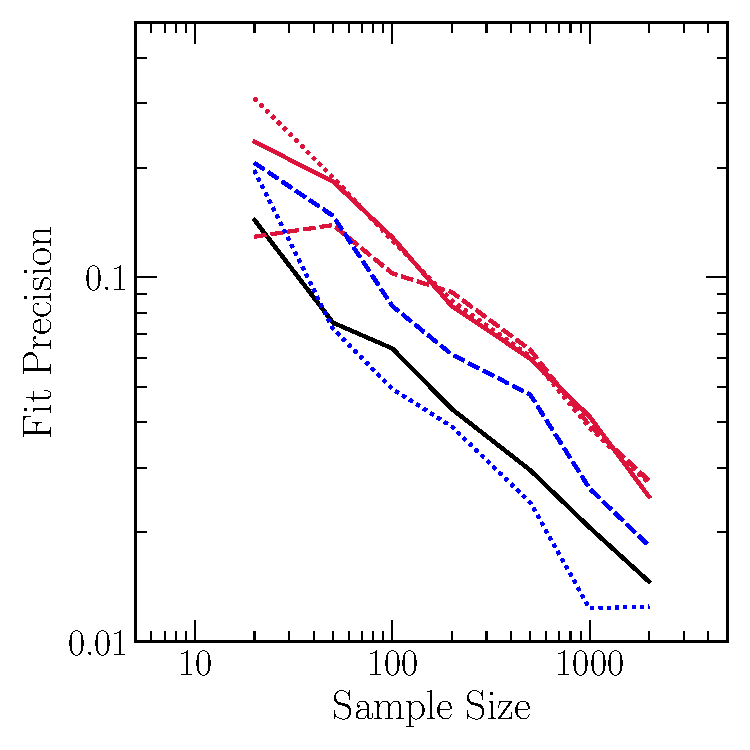
\includegraphics[scale = 0.52]{precision_samplesize.pdf}
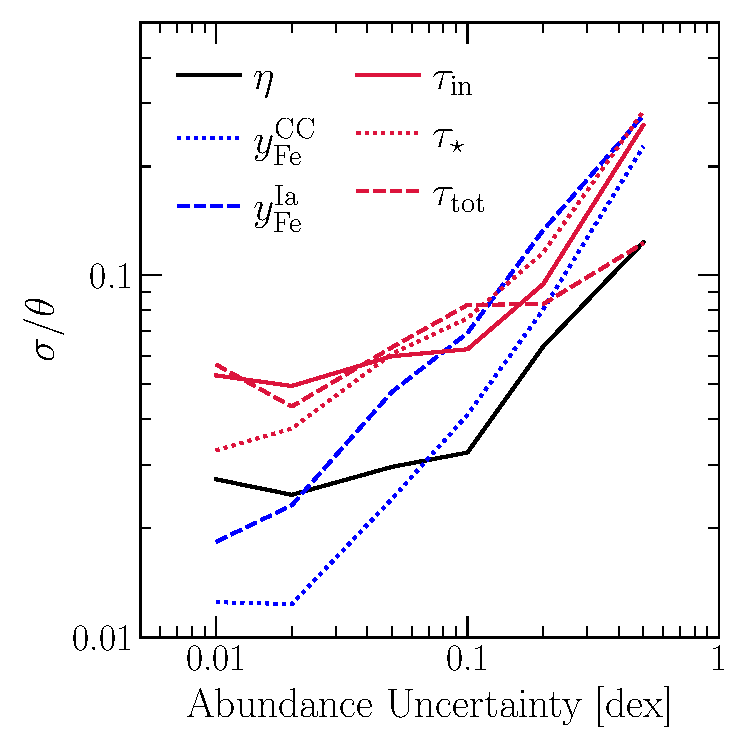
\includegraphics[scale = 0.52]{precision_abundanceuncertainty.pdf}
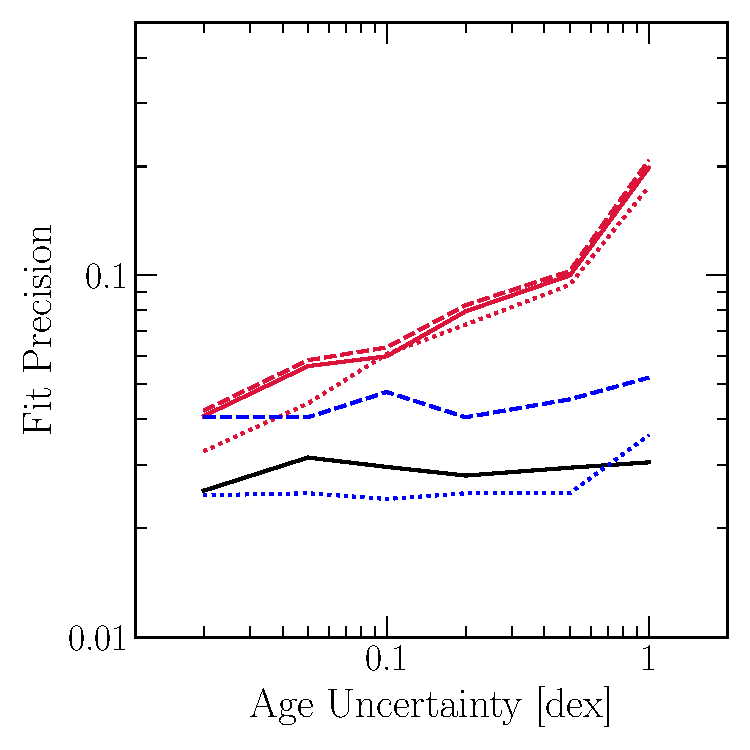
\includegraphics[scale = 0.52]{precision_ageuncertainty.pdf}
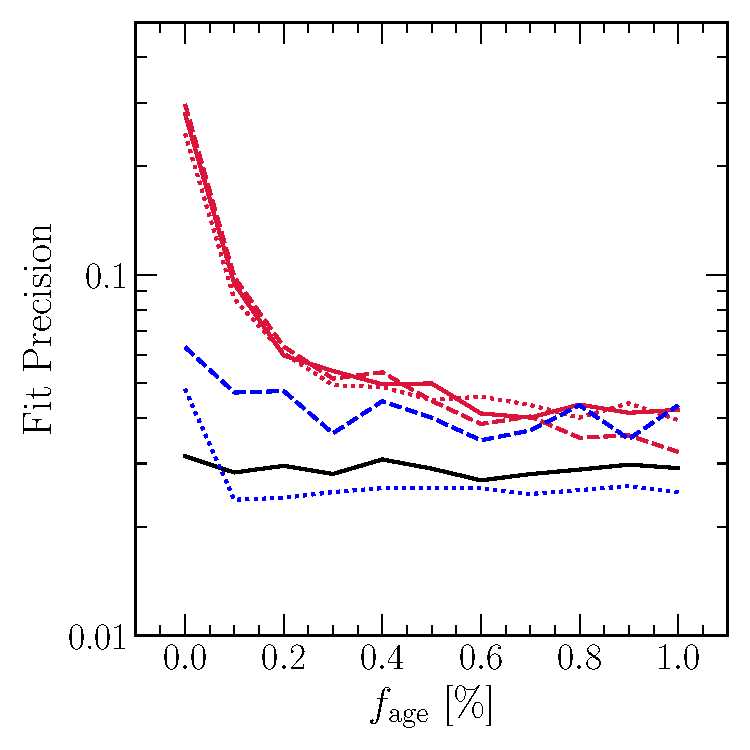
\includegraphics[scale = 0.52]{precision_agefrac.pdf}
\caption{
The precision of our re-derived mock sample parameters~$\{\theta\} =
\{\tau_\text{in},~\eta,~\tau_\star,~\tau_\text{tot},~\yfecc,~\yfeia\}$ as a
function of sample size (top left), measurement uncertainty in~\feh~and~\afe
abundances (top right), measurement uncertainty in~$\log_{10}(\text{age})$
(bottom left), and the fraction of the sample with age measurements (bottom
right).
We plot timescales in red, Fe yields in blue, and the mass-loading factor~$\eta$
in black according to the legend in the upper right panel.
}
\label{fig:precision}
\end{figure*}

	\item These results are of particular interest to authors seeking to derive
	quenching times (i.e. the lookback time to when star formation stopped) for
	dwarf galaxies.
	At present, the most reliable method to empirically determine a dwarf
	galaxy's quenching time is via a direct reconstruction of its SFH through
	some method, such as analysing its CMD~\citep[e.g.][]{Sohn2013, Weisz2015}.
	Consequently, the most precise SFH measurements are for nearby systems with
	resolved stars, a considerable limitation even with modern instrumentation.
	To our knowledge, there are only four quenched galaxies outside of the
	Milky Way subgroup with well constrained SFHs: Andromeda II and Andromeda
	XVI~\citep{Weisz2014a}, Cetus~\citep{Monelli2010a}, and Tucana
	\citep{Monelli2010b}.
	Some authors have connected quenching timescales to observed galaxy
	properties in N-body simulations, (e.g.~\citealp{Phillips2014,
	Phillips2015};~\citealp*{Rocha2012};~\citealp{Slater2013, Slater2014,
	Wheeler2014}), but unfortunately simulation outcomes are strongly dependent
	on the details of the adopted sub-grid models~\citep[e.g.][]{Li2020} as
	well as how feedback and the grid itself are implemented~\citep{Hu2022}.
	Our results suggest that the duration of star formation can instead be
	inferred from the abundances of alpha and iron-peak elements alone, though
	having~\textit{some} age information can significantly improve the
	precision of the fit.
	However, we demonstrate in~\S~\ref{sec:h3:gse} that there are issues that
	arise in practice when comparing to observed data where the functional form
	of the evolutionary history and systematics impacting the data are not
	known exactly.

	% \item Our results suggest that the duration of star formation can instead
	% be inferred from the abundances of alpha and iron-peak elements alone,
	% though having~\textit{some} age information can significantly improve the
	% precision of the fit.
	% However, not only do we fit our mock samples with the exact underlying
	% GCE model, we also use the same numerical code from which the data were
	% drawn to do so.
	% This places the exact same systematic effects on the data as in the model.
	% In~\S~\ref{sec:h3:gse} below, we demonstrate that the age distribution of
	% the GSE is accurately described by our fitting method only when including
	% age information in the fit.
	% Although ages bring little to the table when the exact functional form of
	% the evolutionary history and the systematics impacting the data are known,
	% in practice they bring 

	% \item Our results suggest that the duration of star formation can instead
	% be inferred from the abundances of alpha and iron-peak elements alone,
	% though having~\textit{some} age information can significantly improve the
	% precision of the fit.
	% To benchmark the requirements for deriving these ``chemical quenching
	% times,'' we note from Table~\ref{tab:recovered_values} that our method
	% recovers the duration of star formation with~$\sim$30\% precision with
	% $f_\text{age} = 0$ and with~$\sim$5\% precision with $f_\text{age} = 0.3$
	% for an~$N = 500$ sample, and that this precision scales with the age
	% uncertainties approximately as~$\sigma_{\tau_\text{tot}} / \tau_\text{tot}
	% \propto \sigma_{\log_{10}(\text{age})}^{0.4}$.
	% Furthermore, Fig.~\ref{fig:precision} suggests that the precision of each
	% inferred parameter is affected similarly by sample size, scaling
	% approximately as~$\sigma / \theta \propto N^{-0.5}$.
	% This suggests that deriving the duration of star formation with no age
	% information whatsoever would require~$N \approx 4500$ stars for 10\%
	% precision, but only~$N \approx 180$ for 50\% precision and~$N \approx 45$
	% for order unity precision.
	% However, if only~$\sim$30\% of the sample has age information with
	% $\sim$23\% measurement uncertainty as in our fiducial mock sample (i.e.
	% $\sigma_{\log_{10}(\text{age})} = 0.1$), these scalings suggest that only
	% $N \approx 125$ stars are required to determine the duration of star
	% formation with~$\sim$10\% precision and only~$N \approx 5$ for~$\sim$50\%
	% precision, although the number of degrees of freedom in the model is
	% considerably limited with only~$\sim$5 stars.
	% If the age measurements are instead much more uncertain with only order
	% of magnitude precision (i.e.~$\sigma_{\log_{10}(\text{age})} = 1$), then
	% these scalings suggest that still only~$N \approx 315$ stars are required
	% to derive the duration of star formation with~$\sim$10\% precision and
	% $N \approx 15$ for 50\% precision, though the latter case is again in the
	% regime where the number of degrees of freedom is limited.

	% \item Deriving the quenching time as it is traditionally defined -- the
	% lookback time to the cessation of star formation -- then requires some
	% assumption or knowledge of the lookback time to its beginning.
	% Inspection of the average SFHs predicted by the~\textsc{UniverseMachine}
	% semi-analytic model for galaxy formation~\citep{Behroozi2019} suggests that
	% this generally occurs a little over~$\sim$13 Gyr ago across many decades in
	% stellar mass.
	% The durations of star formation inferred by this method should also
	% be independent of the yield-outflow degeneracy (see discussion
	% in~\S~\ref{sec:mocks:fiducial_fit} and in Appendix
	% \ref{sec:yield_outflow_degeneracy}), meaning that they should be the same
	% regardless of the assumed absolute scale of nucleosynthetic yields and
	% outflows.
	% The feasibility of determining the duration of star formation with minimal
	% or no age information as well as its independence from the yield-outflow
	% degeneracy both arise from the fact that this parameter does not impact the
	% normalization of the MDF, affecting only the shape by cutting it off when
	% star formation stops.
	% With a sample which is sufficient in some combination of size and/or
	% measurement precision, this information can be extracted from the observed
	% MDF.
	% We however caution that the accuracy of this method is contingent on
	% the galaxy in question being accurately described by a one-zone model of
	% chemical evolution.
	% Furthermore, the inferred timescales will be model-dependent and could be
	% inaccurate if the parametrization is a poor description of the galaxy's
	% evolutionary history.
	% Standard quality-of-fit diagnostics such as chi-squared per degree of
	% freedom are a useful litmus test for such cases.

\end{itemize}

\end{document}

